
\chapter{Introduction}
\label{ch:Introduccion}

\section{State of the art}

We will start studying some current devices used for body monotoring as well as their benefits.

Later we will search the methods and experimental procedures used in several studies to analyse of Anticipatory Postural Adjustments in diferents cases, as well as their applications.

Finally, we will speak about the commons calibration techniques, signal processing and classification.


\subsection{Instrumentation}

There are several  device types used to measure APAs. The most importants are: electromyograph, force platform, inertial sensors and devices based on cameras. 

Electromyography (EMG) is a technique that gives us information about the electrical activity produced by skeletal muscles (See figure [1]). The electromyograph can detect  the electrical activity due a electrical potencial difference generated by muscle cells. It’s very useful to analyse posture, locate injuries like muscle paralysis and the place where they are. \cite{Marcio2010} \cite{Instr1}. 


So far, most of realised studies have included like measurement devices, among other things, a platform sensitive to force and pressure. However, the cost and complex of APAs measurement with a traditional movement analysis, using force platform and EMG System limit their applications in the  clinical practice. Therefore, small inertial sensors are used recently because they are cheaper and more portables. But even so, we have used this platform, considering the posibility to ignore it in the future. \cite{Mancini2009} \cite{Vennila2011}.

Devices based in commonly used inertial sensors are IMU (inertial measurement unit), It’s a electronic device that measures and reports about speed, orientation and gravity force of equipment, using the combination of accelerometers and gyroscopes.
In addition, you can combinate it with magnetometers, but in this case, the device is called MIMO. Some current MIMO are: 3DN-GX4-45 \cite{Instr2},  xsens-mvn \cite{Instr3} y mvn-biomech \cite{Instr4}, all of them use Microelectromechanical Systems (MEMS).

\begin{figure}[H]
	\centering
	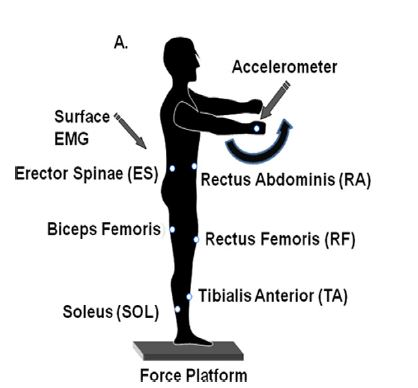
\epsfig{file=imagenes/Captura, width=7cm}
	\caption{EMG, accelerometers y platform \cite{Gay2011}.}
	\label{fig:arte1}
\end{figure}

There are  infrared-reflective markers that give us a complex posture measurement. They are attached  to the body and can provide information about postural strategies, so we can know if the subject uses the ankle strategy or the hip strategy. For example, figure [2] shows the System.

\begin{figure}[H]
	\centering
	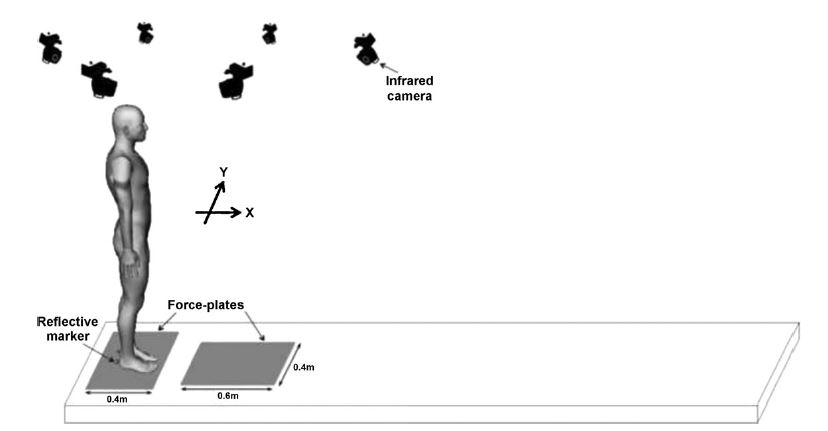
\epsfig{file=imagenes/Captura2, width=7cm}
	\caption{Illustration of the experiment with infrared-reflective markers\cite{Teddy2013}.}
	\label{fig:arte2}
\end{figure}

As mentioned previously, it's possible to use sensors based in cameras that generally are part of a optical System of movement capture such  as Kinect. \cite{Instr5}.


\subsection{Methods and procedure}

So far, a lot of studies about Anticipatory Postural Adjustments are been done, mainly in the  last six years. The finality of the most of this research is be able to deepen knowledge about the posture prior to step initation, and whether there are postural patterns and conditions on which they depend.

If we analyse the state of the art of APAs, we can find that first investigations tried to verify whether APAs are associated to voluntaries movements or no,  this hypothesis was confirmed and the conclusion was it’s more probable that the adjustments don’t appear if step initation isn’t planned. It’s essential for balance control in gait initation because we can use this knowledge to prevent the falls in some people with movement difficults.\cite{Mcllroy1993}\cite{Yiou2012}\cite{Teddy2013}\cite{Bouisset2008}\cite{Neeta2014}

After of this, researchers tried to explain the influence of other variables, such as several exercices that estimulate differents muscles and the reaction of others\cite{Gay2011}; the age influence for generating postural patterns \cite{Bleuse2006} \cite{Estelle2008}; the signal type that initiates the movement ( visual or auditory) due that it affect initial posture \cite{Mcllroy1993}\cite{Antonia2009}\cite{Vicent1999}\cite{Tard2013}; the fear to fall because it can do that patients adopt differents postures[26]; neurodegenerative disease, like Parkinson and Multiple Sclerosis\cite{Mancini2009}\cite{Jebb2008}\cite{Chris2005}\cite{Hall2013}, or cerebral palsy, like hemiplegia and diplegia, \cite{Hall2013}, generate differences in the APAs too.

All these studies are very important in medical applications. For example, As mentioned previously, there are diseases that affect central nervous System, so it affects  the mobility too. Then, it causes falls in many occasions, therefore  the people that suffer the fall have fear of fall again. The fact that fear of fall causes variations in the APAs doing people  fall again, can help us to prevent them.

\subsection{Data Analysis}

In the last years, it has carried out a lot of Works about  calibration of accelerometers and gyroscopes, although the most of them show little variation with others studies done before. One of the most important research  \cite{Kian2011}explains one form to do the calibration putting the acceleromentes in six differents positions and applying  simple algebraic algorithms to the obtained data. The gyroscope is calibrated of different form, using a process based in a known rotation. Also, there are others with the same fundament.

There are other methods that try to be more precise, increasing the number of positions where we record the data \cite{Camps2009}. Also, there are others type of calibration techniques like algorithms based in basic algebraic calculation or in FIR filters. \cite{A.Olivares2013}

As for estimation of orientation for human-body monitoring, if we study the works done so far, we can see that almost all  use a Kalman filter. However, the result with lower signals isn’t very accurate.\cite{A.Olivares2013}

Finally, we will analysis the state of the art of movement recognition in human and classifiers. Quickly, we can see a lot of information about classification because there are a lot of articles and books about this. However, there are others type of studies, which we focus on  it \cite{Banos2012}, that explains methods for human activity recognition based on a sensor weighting hierarchical classifier. This study shows different classification forms that we can use depending on the activities, such as walking or running.

